\documentclass[11pt]{ltjarticle}
\usepackage[b5paper,bmargin=100pt]{geometry}
\usepackage{luatexja}
\usepackage[utf8]{inputenc}
\usepackage{amsmath}
\usepackage{amssymb}
\usepackage{musicography}
\usepackage{leadsheets}
\usepackage{luatexja-ruby} 
\usepackage{wrapfig}
\usepackage{caption}
\usepackage{makecell}
\usepackage{dashrule}
\usepackage{graphicx}
\usepackage{xcolor}
\graphicspath{ {./resources/} }
\usepackage{hyperref}
\usepackage{subcaption}
\usepackage[document]{ragged2e}

\setchords{
    major-seven = \textsuperscript{M7},
    major-nine = \textsuperscript{M9}
}

\renewcommand*\contentsname{目次}
\renewcommand{\figureautorefname}{図}
\renewcommand{\tableautorefname}{表}
\setlength{\RaggedRightParindent}{\parindent}
\setlength{\abovecaptionskip}{0pt plus 3pt minus 2pt}
\RaggedRight
\pagenumbering{roman}
\addtocounter{page}{1}
\setcounter{tocdepth}{2}

%\title{コードオタクが語る東方楽曲分析 \\ \large{第二弾　緋想天 - 砕月からみるメロディーの作り方}}
\author{Metalloid.}
\date{Oct 2025}

\newcommand{\wc}{\writechord}
%\newcommand{\sd}{\textbf}
\NewDocumentCommand{\sd}{}{\musDegree}
\definecolor{bgc}{RGB}{255, 245, 206}


\begin{document}
%\maketitle

{\huge{コードオタクが語る東方楽曲分析}}
\vspace{3pt}
\hrule
\vspace{3pt}
\rightline{\large{第三弾　風神少女から垣間見る\ruby{調}{キー}からの逸脱}}
\vspace{12pt} \rightline{Metalloid.} \rightline{10/2025}

\tableofcontents

\vspace{12pt}
\hrule

\section{まえがき}
どうも、Metalloid.です。前回の砕月でライト回にするとか言いながら文章量が爆発しました。反省しています（解決策は見つかっていません）。と云いつつも、文ちゃん20周年を祝して（去年の京都合同が同人イベント初参加だったという個人的な思い入れもありますが）今回はかなり重たくしたいと思ってしまい、風神少女のハーモニーを分析しようと思い至りました。まぁ、せっかくの京都「合同」なので、サブタイトルを少し秘封っぽくしてみましたが、なにせ自分の中の秘封解像度が低いのでこれくらいで勘弁ください、、\par
前回の寄稿で試し打ちした\LaTeX{}くんはたまに意味不明なことをしますが、それでも便利な子でした。今後ともよろしくお願いしております。\par
\vspace{10pt}
さて、今回の分析のテーマは\ruby{調}{キー}からの「逸脱」、つまり、曲の調に本来含まれず、曲の中で出てくるはずのない局所的アノマリーのような音です。音楽経験があまりない読者のために説明すると、調というのは、曲を書くうえで使用する「制限された音のパレット」であり、一般的に音楽は存在しうるすべての音を使うのではなく、このパレットに従って音を選んで書いていきます（詳しくは付録にて）。風神少女の中では調に収まりきらない音や和音が含まれ、調に忠実に執筆された曲には出せない雰囲気が表現されています。どのような「逸脱」が用いられているのか、そしてそれらがどのように曲と関係しているのか、あるいはどのような効果が生まれるのかを明らかにしていくのが今回の目的です。（もちろんせっかく一曲に焦点を絞っているので、シンプルに和声についてのコメンタリーもするつもりですが。）
\section{分析}
\subsection{概要と構成}
\begin{wrapfigure}{l}{0.4\textwidth}
    \centering
    \vspace{-20pt}
   
\includegraphics[width=0.4\textwidth]{key overview.png} 
   \label{fig:keyOverview}
   \vspace{-15pt}
    \caption{キー概図\cite{circleFifths}}
\end{wrapfigure}
風神少女と云っても、\ruby{東方文花帖}{Bohemian Archive [...]}(8/2005) 、\ruby{東方花映塚}{Phantasmagoria [...]}(8/2005)、\ruby{東方文花帖}{Shoot the Bullet}(12/2005)、\ruby[post=1000]{東方緋想天}{Scarlet Weather [...]}(2008)でバージョンが四つあってややこしいですね。今回主にみていくのは\ruby{東方花映塚}{Phantasmagoria [...]}バージョンです。長尺の方にしない主な理由として、今回の観点である和声の面からすると、長尺と短尺とであまり違いがないという点があります。\par
曲の構成は以下のようで、ポップス曲のようにサビが複数回登場するようにできています。今回はコード進行についてみていこうと思うので、反復の分は特に事情がない限り触れないようにします。
\begin{multline*}
    \text{イントロ $\rightarrow$ \leftrepeat　間奏$\rightarrow$Aメロ$\rightarrow$サビ$\rightarrow$ 間奏} \\ \text{$\rightarrow$ Aメロ $\rightarrow$ サビ $\rightarrow$ 落サビ $\rightarrow$ ラスサビ　\rightrepeat}
\end{multline*}
調の移ろいも単純で、落サビでFmからF\sh mへの半音転調がみられます。


\subsection{イントロ\&間奏}
\begin{figure}
    \centering
    
\includegraphics[width=0.9\linewidth]{resources/intro.png}
    \caption{イントロ概譜}
    \label{fig:intro}
\end{figure}
\begin{figure}[]
    \centering
   % \vspace{-60pt}
    \fcolorbox{black}{bgc}{
        \begin{minipage}{\linewidth}
        \textbf{アンダルシア進行} \\ ローマ数字で記述するなら、\wc{i bVII bVI V}。スペインのフラメンコ音楽が起源である。学者によっては、歴史的文脈に於いてこの進行をフリジアン音階における\wc{iv bIII bII I}と評価し、最後のコードをトニックとして解釈する者もいる。今回はそのような用法ではなく、一つ目のコードがトニックとなっている。
        \end{minipage}
    }
\end{figure}
\begin{wrapfigure}{r}{0.4\textwidth}
    \centering
    \vspace{-20pt}
    \fcolorbox{black}{bgc}{
        \begin{minipage}{\linewidth}
        \textbf{アルペジオ} \\ 
        コードの構成音を、時間の中で分散して鳴らすフレーズ
        \end{minipage}
    }
\end{wrapfigure}
イントロでは、四小節の間ズンペとベースが存在し、その後他の楽器が参入し曲が本格的に始まります（\autoref{fig:intro}）。最初の四小節のズンペのメロディーはコードのアルペジオであり、音をとってみると明らかな形で\wc{Fm} \wc{Eb} \wc{DbM7} \wc{C}のコード進行（アンダルシア進行ともいう）を形成していることがわかります。それに対して、ベースは歯切れの良い音を織り交ぜながら高速で周辺を駆け巡っているようで、特にズンペの作るコードと整合するような動きをしていません（一小節目のズンペのE\na に対するベースのE\fl 等）。このベースフレーズのピッチを通常再生速度で正確に聞き取ることはかなり困難なので、その衝突が気づかれずに済むということも言えます。\par
最初の四小節を経て、曲は間奏の提示を行います。ここではアンダルシア進行が継続されており、途中からピアノの高速フレーズが入ります（\autoref{fig:introPiano}）。このフレーズは\autoref{fig:intro}の3～4小節目のズンペを大方再利用したものです。\par 




\begin{figure}
    \centering
    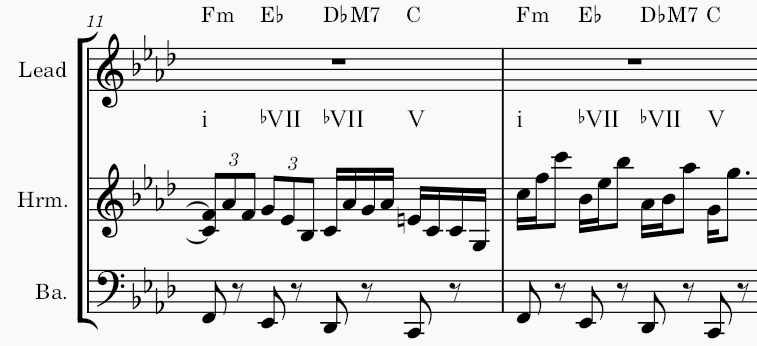
\includegraphics[width=0.9\linewidth]{resources/intro piano.png}
    \caption{イントロピアノ}
    \label{fig:introPiano}
\end{figure}
\vspace{15pt}
最後に、一番と二番の間の間奏に少し触れようと思います。
\begin{figure}
    \centering
    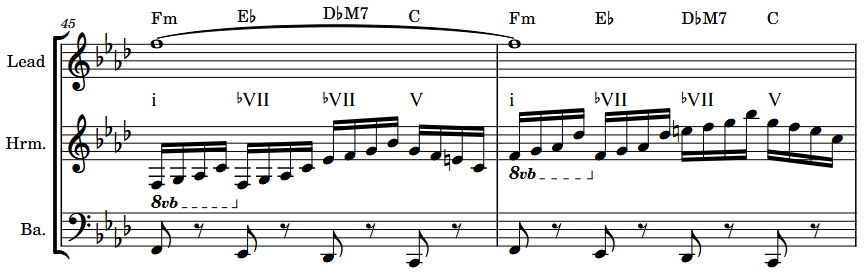
\includegraphics[width=0.9\linewidth]{resources/bridge piano.png}
    \caption{一二番間奏ピアノ}
    \label{fig:bridgePiano}
\end{figure}
ベースがアンダルシア進行を敷いているうえで、ピアノの速弾きが流れます（\autoref{fig:bridgePiano}）。この速弾きはシンプルな構造をしていて、二小節パターンを反復しながら、後半では前半の分を一オクターブあげて焼き直しています\footnote{ちなみに、同じピアノ速弾きを、オクターブを変えて再利用するという手法は亡き王女の為のセプテットでもみられます。}。一小節目では二拍分\wc{Fm} (厳密には\wc{ Fmadd9})のアルペジオを鳴らした後、進行三拍目の\wc{Db(M7)}に対してE\fl からB\fl に向かって上昇し、\wc{C}に対しては（経過音を踏みつつ）\wc{C}のアルペジオのようなフレーズを弾いています。二小節目では、二拍分\wc{Db} (厳密には\wc{Db(#4)})のアルペジオを鳴らした後、三拍目でE\fl ではなくE\na からB\fl まで上昇しています。\par
これらのピアノの音は下に敷かれているコード進行とはかなり無関係な動き方をしていますが、敢えてコードシンボルを当てるとするならば\wc{Fmadd9 Eb13 Db(6/9#4) C7 Fm(b6) Eb13 Db(6#9#4) C7}のようなものになります。ここまでくるとかなり無意味なコードシンボルになるので、個々の音が聞き取りずらいピアノ速弾きはこの箇所のコード譜に反映していません。ただ、一か所だけ明確に目立つところがあります。それはE\na です。\par
E\na はこの部分でのキーであるF短音階に含まれず、代わりにFから作る、暗い\ruby[pre=1000,post=1000]{和声短音階}{ハーモニックマイナースケール}に含まれます。そのため、E\na が登場することにより暗さが発生します。それ以前に、キーに含まれながらも不安定な響きを持つD\fl の音も踏んでいることから、この小節から暗めの雰囲気が滲み出るのです。


\subsection{Aメロ}
\begin{figure}
    \centering
    
\includegraphics[width=0.9\linewidth]{resources/verse.png}
    \caption{Aメロ}
    \label{fig:verse}
\end{figure}
\autoref{fig:verse}でみえるように、Aメロではアルペジオ型のシンプルなメロディーおよびベースが、\leftrepeat \wc{Fm Eb} \wc{Dm} \rightrepeat（ローマ数字なら \leftrepeat \wc{ i bVII vi} \rightrepeat）というコード進行を示しています。3～4小節に渡って登場する\wc{Dm}は、\autoref{fig:verse}での臨時\na 記号の数からも見えるように、キーに存在しないコードで、独特な雰囲気を醸し出します。僕ならここから秋の臭さを感じますね。このコードパターンを二週してから次はキーの中にしっかりと存在するコードパターン(\wc{Db} \wc{Eb} \wc{Fm})が登場します。これは東方やjpopでお馴染の、全音上がりの\wc{bVI bVII i}進行ですね。\footnote{厳密に登場したのは\wc{Fm}ではなく\wc{Fm/C}であるので、完全に例の進行として感じられるかというと、異論は認められます。}\par
\vspace{15pt}
さて、踏み込んだ話をしてみましょう。キーから逸脱しているはずの\wc{Dm}が、なぜそこまで不自然に聞こえないのでしょうか。これにはいくつかの理由がありますが、大きく考えて二つの主な要因があると思います。
\begin{enumerate}
    \item ベースの動き方が、東方で頻出のパターンに沿っている
    \item \wc{Dm}と\wc{Fm}のコードの間に近親さがある
\end{enumerate}
まず、1.について。キーから逸脱しないとするならば、ベースが\sd{1} (今回ならF)を鳴らしたあと、\fl \sd{7} (E\fl )を経て\fl \sd{6} (D\fl )を踏むのが予想できます。しかし、今回は\sd{1} \fl \sd{ 7}を踏んだのち、\na \sd{6} (D\na )を踏んでいますね。実は\sd{1}, \fl \sd{7}から\na \sd{6}を踏むこと「自体」はZ氏の常套句で、風神録5面道中-少女が見た日本の原風景（公式音源0:32～0:36）、文の妖怪の山〜Mysterious Mountain（公式音源0:13～0:16）や、最近の曲ならば錦上京2面のセイクリッドフォレスト（音源0:22～0:30\cite{FWOST}）でみられます。\footnote{ただ、これらの例では、そのベースを用いて作るコードが今回と異なります。具体的にいうと、これらは風神少女でみられる\wc{vi}ではなく、\wc{IV}/\na \sd{6}を形成します（\autoref{fig:verseBass}）。これが生む大きな違いとして、\wc{IV}がキーのなかでサブドミナントとして機能するのに対し、\wc{vi}はトニックでもドミナントでもサブドミナントでもなんでもない、無機能的なコードであるという点です。}\par
\begin{figure}
    \centering
    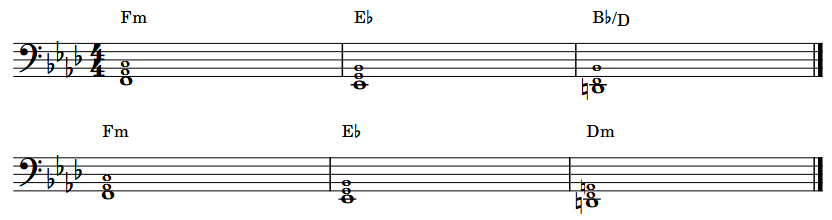
\includegraphics[width=0.9\linewidth]{resources/verse bass.png}
    \caption{上：少女が見た日本の原風景のイメージ　下：風神少女のイメージ}
    \label{fig:verseBass}
\end{figure}
次に、2.について。\wc{Dm}と\wc{Fm}は、共有する短音階を持たず、\wc{Dm}は絶対にキーの外へと出てしまうのに、いざ曲の中で聞いてみると、そこまで「逸脱した」「ハズした」ような匂いはしません。その根本原因となるのが、\wc{Dm}と\wc{Fm}のルートが三度離れであるということです。\par
ルートが三度離れのコードはサウンドから役割まで、かなり似ると云われます。簡単な例だと、\wc{C}と\wc{Am}や\wc{C}と\wc{Em}は似ていると云えます。その原因はそれぞれCとE、EとGを共通の音として持っているからです。では、\wc{C}と\wc{E}のような、ルートが三度離れであっても、共通のキーがないようなコードはどうでしょうか。E音は共通していますが、片方がG\na を使うのに対し、もう片方はG\sh を必要とします。見かけ上は共通音が多いはずなのに、G\na かG\sh か、どっちのバージョンを使うべきか喧嘩しているかのようです。このような関係を\textbf{クロマチックメディアント}と呼びます。クロマチックメディアントはルートが三度離れであるためにどこか「似ている」という性質がありながらも、どこか決定的なところで相違点を持つ組み合わせで、今回の\wc{Dm}と\wc{Fm}のペアはこの関係性に当たります。つまり、この二つのコードが、キーを違えていても、どこかで「十分に似ている」おかげで、曲の中で浮かないで済むと云えます。
\begin{figure}
    \centering
    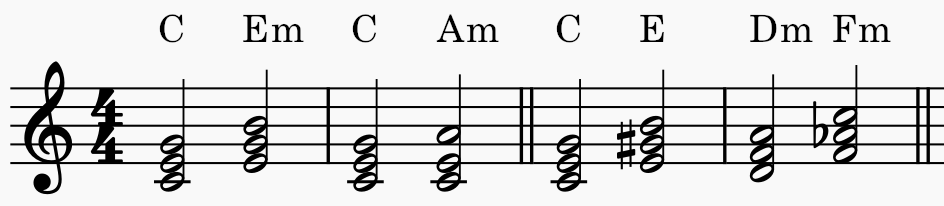
\includegraphics[width=0.9\linewidth]{resources/mediants.png}
    \caption{左：メディアント関係、右：クロマチックメディアント関係}
    \label{fig:mediants}
\end{figure}
\begin{figure}[b]
    \centering
   % \vspace{-60pt}
    \fcolorbox{black}{bgc}{
        \begin{minipage}{\linewidth}
        \textbf{クロマチックメディアント} \\ ルートが三度離れで、共通音を一つしか持たないコード。調性を前提としない理論体系で頻繁に見る。
        \end{minipage}
    }
\end{figure}
\par\vspace{15pt}
さらに深堀すると、クロマチックメディアント等、スケールを前提としないコードの関係性をまとめた理論として、\textbf{ネオリーマン理論}が存在します。これ以上原稿本編の面積を独占してはいけないので、付録にて少し詳しく説明します。
\par\vspace{15pt}
さて、Aメロの最後は緊張感を高めるために\ruby[pre=1000,post=1000]{和声短音階}{ハーモニックマイナースケール}を用いて\wc{C} (\wc{V})和音を鳴らして、サビに渡ります。
\begin{figure}
    \centering
    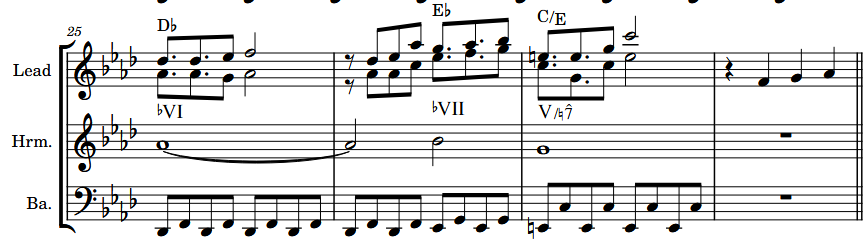
\includegraphics[width=0.9\linewidth]{resources/prechorus.png}
    \caption{Aメロとサビの繋ぎ}
    \label{fig:preChorus}
\end{figure}
\subsection{サビ}
\subsubsection{セクションの流れ}
サビの構成は簡単な起承転結構造をとっており、基本的なパターンは\autoref{fig:chorus}のようになります。\wc{bVI} \wc{bVII} \wc{i}進行を基本構造としたうえで、反復によってメロディーを形成しています。サビを通してこのコード進行は基本的に変わらないのですが、三回し目のみ、変化球（公式音源1:01）が入ります(\autoref{fig:chorusInterchange})。\wc{Db} \wc{Eb} \wc{Fm}と、\wc{Fm}に着地する代わりに、\wc{Bb/D}\na からの\wc{C7/E}\na を通り、（読みやすさのためにベースの動きを省略すると）\wc{bVI} \wc{bVII} \wc{IV} \wc{V7}という進行を踏みます。この段階で、臨時\na から見えるように、本来の音階から逸脱した音が続いて使用されます。しかし、いずれの場合も、本来キーの中でマイナーコードとして存在するべきであったものをメジャーコードに変換するための逸脱なので、そこまでおかしく聞こえません。\par
\subsubsection{変化球の\wc{IV} \wc{V}の素性と効果とは？}
先述の「変化球」、すなわちこの\wc{Bb/D}\na と\wc{C7/E}\na の二つのコードが、曲の中で印象に残るかなり特異的な点であることは確かです。では、これらは理論的にはどういう意味があるのか、どのような効果が生み出されているのかを見ていきましょう。それをするにあたって、これらは元来の調に存在しない外来コードなので、一体どこから生まれたのかを考えるというのが一つの手段です。このコードたちが一体どこから誕生したのかについて、この段階でいくつかの仮説を建てることができます。（表記簡単のため、ここからベース記号を省略し、\wc{Bb}、\wc{C7}と表記する。）\par
\begin{figure}
    \centering
    
\includegraphics[width=0.9\linewidth]{resources/chorus.png}
    \caption{サビの最初の四小節}
    \label{fig:chorus}
\end{figure}
\begin{figure}
    \centering
    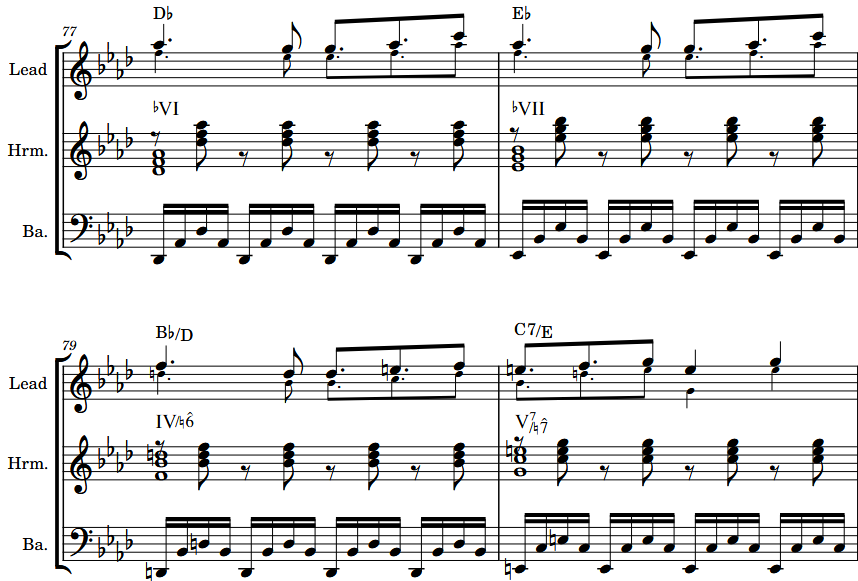
\includegraphics[width=0.9\linewidth]{resources/chorus interchange.png}
    \caption{サビの三周目}
    \label{fig:chorusInterchange}
\end{figure}
\begin{enumerate}
    \item 長音階説：FマイナーからFメジャーへと、短調から長調へ局所的に転調した。
    \item ドリアン説：Fドリアンスケールから\wc{Bb}を借用し、次の小節でFハーモニックマイナーから\wc{C7/E}を連れてきた。
    \item 旋律短音階説：F\ruby[pre=1000,post=1000]{旋律短音階}{メロディックマイナースケール}から\wc{Bb}も\wc{C7}も両方取ってきている。
\end{enumerate}
それぞれの仮説では\wc{Bb}および\wc{C7}がどのスケールから来ているのか、つまり、これらのコードによってどのような音階の風味が想起されるのかが違います。それぞれの仮説の意味すること、およびその信憑性を一つずつ見ていくことにより、この２つのコードがこの楽曲でどのような効果を生み出しているのかに迫ろうという試みです。\par
\vspace{10pt}
\textbf{長音階説}\\
この箇所で曲が短調から長調へ転調したとするなら、Fメジャーから借用された\wc{Bb}と\wc{C7}は長調の明るさを宿すはずです。実際に原曲を聴いてみると、\wc{Bb}は明るいとも言えなくもないですが、\wc{C7}（譜上80小節・公式音源1:02）には明るさの欠片もありません。むしろ、緊張感が高まり、サビの四回し目への期待が溢れそうな、極めて不安定な二秒間です。これでは、この箇所が「長調」らしく、明るく聞こえるとは言えません。つまり、\wc{Bb}および\wc{C7}がFメジャーからの借用であり、この箇所で調性が短調から長調へ部分転調したという仮説は些か弱いということです。\par
\vspace{10pt}
\textbf{ドリアン説}\\
ドリアンスケールは、自然短音階のうち一音を半音上げることによって生まれる新しい音階で、一つの特徴として、自然短音階のダイアトニックコードの一つである\wc{iv}がマイナーコードからメジャーコードへと変化し、\wc{IV}になるという点があります。ドリアンスケールはよく、短調のもの寂しげな響きを残しながらも、その中で希望の存在を仄めかすような、比較的明るめの音階として知られています。今回にあてはめると、Fマイナースケールの構成音はF, G, A\fl , B\fl , C D\fl , E\fl であるのに対して、Fドリアンの構成音はF, G, A\fl , B\fl , C, D\na , E\fl になります。ここから、確かにB\fl , D\na , Fを取ってくることにより件の\wc{Bb}コードを作り上げることはできます。\par
\begin{figure}[]
    \centering
   % \vspace{-60pt}
    \fcolorbox{black}{bgc}{
        \begin{minipage}{\linewidth}
        \textbf{ドリアンスケール} \\ 
        \begin{wrapfigure}{r}{0.3\linewidth}
            \centering
            \vspace{-25pt}
            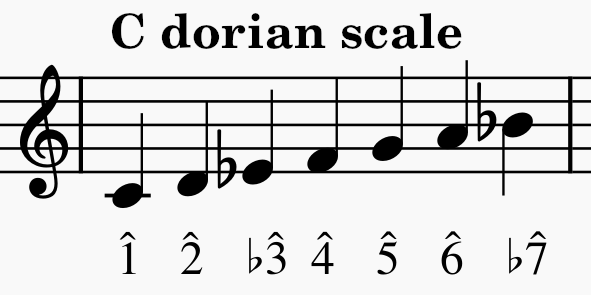
\includegraphics[width=\linewidth]{resources/dorian scale.png}
            \caption{Cドリアンスケール}
            \label{fig:dorian}
        \end{wrapfigure}
                自然短音階の\fl \sd{6}度を半音上げることによって生まれる新しい音階で、比較的明るめなサウンドを持つ。主に短調で\wc{IV}を使うために活用されるが、たまに\wc{ii}のためにも使われることもある。世の中では、よく「中世風RPGの宿屋のBGM」っぽい音階として評される。
        \end{minipage}
    }
\end{figure}
確かに、この\wc{Bb}（譜上79小節・公式音源1:01）は明るく聞こえ、一気に楽曲が空へと持ち上がっていることは確かであるので、この効果を「ドリアンスケール由来の\wc{Bb}により、その明るさが輸入された」と説明することは可能です。\par
ちなみに、比較用に　この\wc{Bb}の代わりに調から逸脱しない\wc{Bbm}を使ってみた簡易音声を作ってみました。やはり、普通の短音階に忠実に曲を書いて\wc{Bbm}を用いた場合、短音階から逸脱して\wc{Bb}を用いた原曲より幾分か暗くなるので、この「明るくなる」といった効果は事実として存在すると思います。
\par
最後の点として、他にも射命丸文関連の曲として妖怪の山の中でも、短調文脈の中での一時的なドリアンスケール借用による明転アクセントがみられます：
\begin{itemize}
    \item イントロの最後の２小節（公式音源0:15~0:17）
    \item Aメロ6小節目（公式音源0:22）
\end{itemize}
ここから、空を軽々しく舞うことのできる文のキャラクター表現としてドリアンスケールの、この空中に持ち上がるような明るさが用いられているという結論を導くのは不自然ではないと思います。\par
\vspace{10pt}
しかし、実際に風神少女の採譜を行って楽譜にまとめ、79小節目の中身を丁寧に吟味したところ、この説明では納得の行かない音が一つメロディーに含まれていることが明らかになります。それが、同小節メロディーに登場する２つ目の\musEighthDotted の、E\na の音です。先程Fドリアンスケールの構成音を羅列しましたが、ドリアンスケールにはE\na は含まれず、E\fl を使用しなければならないことになります。つまり、この小節全体で考えると、ドリアンスケールのみが用いられたとは云えません。\par

\vspace{10pt}
\textbf{旋律短音階説}\\
音楽経験のある読者、または付録を読んでくださった方なら和製短音階のことを認知していると思います。旋律短音階というのは、伝統的には和声短音階の六度目を、自然短音階からドリアンスケールへの変換と同様にして、半音あげることによって得られる音階です。つまり、Fから構成音を順番に構築していくと、F, G, A\fl , B\fl , C, D\na , E\na になります。ここでポイントになるのが、ドリアンスケールの場合と同様に、F, B\fl , D\na が共通して存在しているので、\wc{Bb}コードの由来として、この旋律短音階も有効な選択肢であることです。そして、この音階は79小節目のメロディーで存在していたE\na を確かに含んでいます。また、和声短音階と同様にG, B\fl, C, E\na を含んでいるので、続く80小節の\wc{C7}を十分説明する力があります。まとめると、79小節から80小節にかけて、この「変化球」は旋律短音階の使用から生まれたという説明は十分に妥当です。この考え方を追うならば、79小節目で旋律短音階が使用され\wc{Bb}が打たれる理由として、80小節目での旋律短音階に合わせるため、という読みができます。\par
それでは旋律短音階がどのような雰囲気を放つのかについてですか、基本的に旋律的短音階がドミナントコードとともに使われる場合が多いため、不安定で緊張感のある音階として捉えることもできます。しかし、旋律短音階が長音階と多くの共通音を持つことから、場合によっては明るい音階としても捉えらるので、ドリアンスケールの時ほど簡単に「これといった雰囲気」を名指しすることは難しいです。\par
\par
\begin{figure}[]
    \centering
   % \vspace{-60pt}
    \fcolorbox{black}{bgc}{
        \begin{minipage}{\linewidth}
        \textbf{旋律短音階} \\ 
        \begin{wrapfigure}{r}{0.35\linewidth}
            \centering
            \vspace{-25pt}
            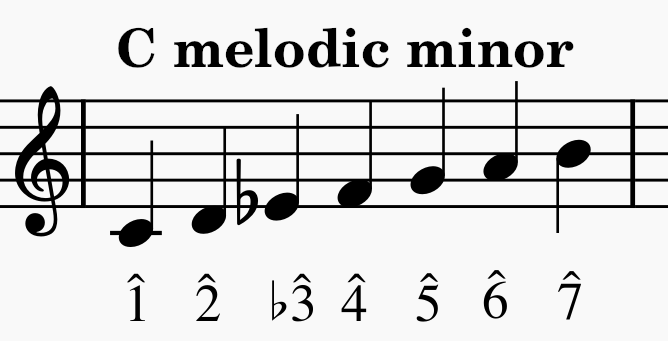
\includegraphics[width=\linewidth]{resources/melodic minor.png}
            \caption{C旋律短音階}
            \label{fig:dorian}
        \end{wrapfigure}
        メロディックマイナースケールとも。和声短音階の\fl \sd{6}と\na \sd{7}の間の三半音の音程が広すぎるという理由から、旋律を書く上でその\fl \sd{6}も半音上げて\na \sd{6}にしよう、という発想が起源。\wc{V}に対して使用されることが多い。
        \end{minipage}
    }
\end{figure}
\vspace{10pt}
\hdashrule[0.5ex][c]{0.5\linewidth}{0.5pt}{1.5mm}
\par
\textbf{以下オタク向け注}\\
先ほど旋律短音階が用いられたことによって\wc{IV}および\wc{V7}が発生したという説明の仕方を試みましたが、僕の調べた範囲ですと旋律的短音階の用途は和声短音階と同様に\wc{V7}(\wc{V9})の形成が多いようで、今回のようにプレドミナントの形成のために使われるのはもう少し稀であると思います。\par
旋律短音階が和声短音階の代わりに使用される例として、イギリス民謡のGreensleevesという曲があります。一見して普通の曲ですが、一か所で\wc{V}の上に\na \sd{7} \na \sd{6} \na \sd{7}というメロディーが載ります（\autoref{fig:greensleeves}）。一般的な和声短音階使用では\fl \sd{6} (F)を使うところですが、この曲では敢えて\na \sd{6} (F\sh )が\wc{V}の上でアクセントのように使用されております。\par
\begin{figure}
    \centering
    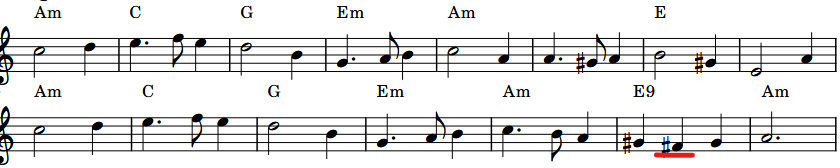
\includegraphics[width=0.9\linewidth]{resources/greensleeves.png}
    \caption{Greensleeves譜例}
    \label{fig:greensleeves}
\end{figure}
また、J.S.バッハの曲の中では、\wc{i}や\wc{V}に対しては旋律短音階の使用が見られたのに対し、サブドミナントコードに対してはあまり確認されなかったという研究も存在します\cite{bachMMS}。\par
\hdashrule[0.5ex][c]{0.5\linewidth}{0.5pt}{1.5mm}
\par
\vspace{10pt}
\textbf{議論の結論として}\\
風神少女のサビの三回し目に登場する「変化球」、すなわち\wc{Bb/D} \wc{C7/E}は、明るい長調への部分転調であるとは云えません。\wc{C7/E}は素性がシンプルで、緊張感のあるコードとして旋律短音階借用により発生したものとして捉えることができますが、\wc{Bb/D}の方は所説あり、文の他のテーマ曲でみられるようなドリアンスケールへの一時的な明転として考慮することもできれば、採譜を第一に信じ、旋律短音階の現代的活用法として考えることもできます。これらを融合しようとするならば、小節の最初ではドリアンスケールの明るさを主張しつつも、小節の途中から少しずつ雰囲気を変化させ、次の小節の緊張したコードを導く、という構成の読みができます。
\subsection{まとめ}
長くなりましたが、話をまとめあげようと思います。風神少女ではわかりやすい楽曲構成の中で、度々調から逸脱した音や和音が使われています。\par
その一つがAメロの三小節目で見られる\wc{Dm}で、これは完全に調から逸脱した和音でありながらも、調の中で最も安定な和音であるトニックコード\wc{Fm}と近親的であるがために、曲の中に溶け込むことができています。\par
もう一つの逸脱はサビの三回し目で毎回登場する二つのコードで、そのうち後者は緊張感を高める作用を持つのに対し、前者はちょっとした明るさを持ち合わせながらも、次の緊張したコードへとシームレスにバトンを繋げる役目があると分析することが可能です。
\section{付録}
\subsection{音楽理論基礎 (再掲)}
以下は基本的に前回の付録にマイナーチェンジを施したものです。\par 
執筆途中の段階で、音楽を知っている方でも、音楽理論をしらないとこの文章を読んでいても何も楽しくもないのだろうなと気づき始めたので、“ダイジェスト版“で基本的な音楽理論の概念を付録に載せようと思い至りました。といっても、簡潔な文章を書くのが苦手なので、本当にダイジェストになるかはわかりません。ごめんなさい。
\subsubsection{半音階}
ピアノや鍵盤をみたことがある人ならわかると思いますが、一オクターブの中には12個の音があります。ソルフェージュではこれらをド, ド\sh /レ\fl , レ, レ\sh /ミ\fl , ミ, ファ, ファ\sh /ソ\fl , ソ, ソ\sh /ラ\fl, ラ, ラ\sh /シ\fl , シと呼びますが、僕はブリティッシュインペリアリズムに負けた人なので、これらをC, C\sh /D\fl , D, D\sh /E\fl , E, F, F\sh /G\fl, G, G\sh /A\fl , A, A\sh /B\fl , Bと呼びます。特別に和な心持でこれを読まれている方はきっと心の中ではハ, 嬰ハ/変ニ, ニ, 嬰ニ/変ホ, ホ, ヘ, 嬰ヘ/変ト,ト, 嬰ト/変イ, イ, 嬰イ/変ロ, ロと呼んでいるのでしょう。若かりし4.5年前の自分の抱いた疑問にて、B\sh とE\sh , C\fl とF\fl は一体どこにいったのだ、という問いがありましたが、これはピアノの鍵盤をみたらわかります。E\sh =Fなのです。\textbf{ただし、これは近代的なチューニング体系を用いる音楽に限られ、本来C\sh とD\fl は異なる音、B\sh とCも異なる音であると考えられていました。}半音階で隣接した二つの音の差を半音、二半音の差を全音と呼びます。つまり半音は世に出くわすほとんどの音楽においてはピッチの距離の最小単位となります。
\subsubsection{音程}
音程をピッチの同義語だとよく思われますが、厳密にはそれは嘘で、辞書的には「二つの音のピッチの距離」を意味します。音程の言葉の例としては「完全五度」「長六度」「短三度」などがあり、何かしらの「質」と「数」が組み合わさっています。音程の「数」は二つの音の間にまたぐアルファベット種の数、楽譜上での線（と空白）の数、あるいは鍵盤上の跨ぐ白鍵の数と認識すると良いでしょう。ただし、1から数えられます。\par
例：
\begin{itemize}
    \item \textbf{A}と\textbf{C}はA, B, Cの三文字を跨ぐので、\textbf{三度}の距離があります
    \item \textbf{F}\sh と\textbf{D}\sh はF, G, A, B, C, Dの六文字を跨ぐので、\textbf{六度}の距離があると云えます
\end{itemize}\par
しかし、このままでは問題があります。例えば、CとEとの間の音程は三度であるといえます。同様に、DとFの間も三度の差があります。しかし、それぞれの距離を半音ベースで数えると（0から数えて）CとEは四半音差、DとFは三半音差です。つまり、音程の「数」では実際の音の距離を一意的に決定・記述することができないのです。そのために、音程の言葉には「質」が接頭辞としてつきます。これは「長」「短」「増」「減」「完全」の五種あり、
\begin{enumerate}
    \item 歴史的経緯から(ユニゾン(0半音)、オクターブ(12半音))、7半音の「五度」、5半音の「四度」には「完全」がつきます。（ただ、六半音の音程については別名の「トライトーン」が存在します）
    \item それ以外では、白鍵だけを考えたときに総当たりを行い、「デカい」に「長」、「小さい方」に「短」がつきます。
    \item 上のスキームに当てはまらなかったものに対して、「減」と「増」がつきます：
    \begin{itemize}
        \item 完音程や長音程を一半音広めるときに「増」
        \item 完音程や短音程を一半音狭めるときに「減」
    \end{itemize}
\end{enumerate}
いきなりルールを説明されても難しいと思うので、実例をみてみましょう。
\begin{itemize}
    \item \textbf{A}と\textbf{G}の間は、A B C D E F Gの七種の文字が存在し、半音距離は10なので、\autoref{tab:intervals}を以て短七度の距離であるといえる
    \item \textbf{A}と\textbf{F}\sh の間では、A B C D E Fの六種の文字が存在し、半音距離は9なので、長六度の距離である
    \item \textbf{A}と\textbf{E}の間は、A B C D Eの五種の文字が存在し、半音距離は7なので、\autoref{tab:intervals}を以て完全五度の距離であるといえる
    \item \textbf{A}と\textbf{E}\fl の間では、A B C D Eの五種の文字が存在するが、半音距離は6であるので、上記の完全五度を狭めたものであるとして、減五度(\autoref{fig:intervals}参照)であると云える。また、この場合は慣用名のトライトーンという言葉も使うことができる。
    \item \textbf{A}と\textbf{D}の間では、A B C Dの四種の文字が存在し、半音距離は5なので、完全五度の距離である
    \item \textbf{A}と\textbf{D}\sh の間では、A B C Dの四種の文字が存在するが、半音距離は6であるので、上記の完全四度を広めたものであるとして、減五度(\autoref{fig:intervals}参照)であると云える。また、この場合は慣用名のトライトーンという言葉も使うことができる。
    \item \textbf{A}と\textbf{G}\fl の間では、A B C D E F Gの七種の文字が存在するが、半音距離は9であるので、上記の短七度を狭めたものであるとして、減七度(\autoref{fig:intervals}参照)であると云える。（G\fl はF\sh と「同じ」であるとして、長六度として丸めてしまいたいと思うかもしれないが、命名のルールと、冒頭で述べたようにそもそもF\sh とG\fl という音符が同じピッチを指すとは限らないことから、長六度という名前は原理的には不適切である。）
\end{itemize}
\begin{figure}
    \begin{subfigure}{0.4\textwidth}
        \centering
        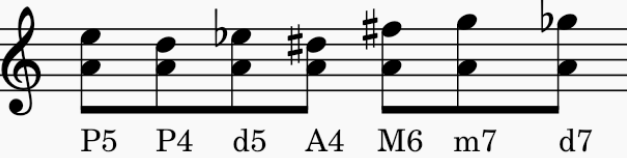
\includegraphics[width=1\linewidth]{resources/intervals.png}
        \caption{音程例}
        \label{fig:intervals}
    \end{subfigure}
    \begin{subfigure}{0.5\textwidth}
        \centering
        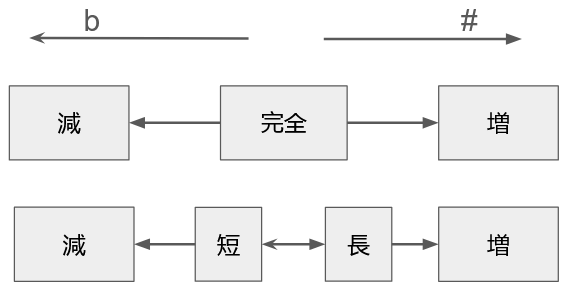
\includegraphics[width=1\linewidth]{resources/interval quality.png}
        \caption{音程の質}
        \label{fig:音程の質}
    \end{subfigure}
    \centering
    \caption{音程について}
\end{figure}
\begin{table}
    \centering
    \caption{基本的音程名}
    \begin{tabular}{|c|c|c|c|}\hline
        半音距離 & 和名 & 英名 & 略\\ \hline
        0 & ユニゾン &  (Perfect) Unison& P1\\
        1 & 短二度 &  Minor Second& m2\\
        2 & 長二度 &  Major Second& M2\\
        3 & 短三度 &  Minor Third& m3\\
        4 & 長三度 &  Major Third& M3\\
        5 & 完全四度 &  Perfect Fourth& P4\\
        6 & トライトーン&  Tritone& TT\\
        7 &  完全五度 &  Perfect Fifth& P5\\
        8 &  短六度 &  Minor Sixth& m6\\
        9 &  長六度 &  Major Sixth& M6\\
        10 & 短七度 &  Minor Seventh& m7\\
        11 &  長七度 &  Major Seventh& M7\\
        12 &  オクターブ &  (Perfect) Octave& P8\\\hline
    \end{tabular}
    \label{tab:intervals}
\end{table}
覚えることが大変かもしれませんが、これだけ押さえておけば基本的にはあとあともう困らないと思います。
\subsubsection{コード}
コードというのは最も基本的な理解ではある音（ルート）の上に三度を順番に積み重ねて作るものです。では色々組み合わせて作っていきましょう。三度の種類は二種類あったので、音を三つ使ったコードは4パターンありえます。（\autoref{fig:triads}）コードの命名は、ルートの上に何がくるかによって決定されます。例えば、右から二つ目はルートの上にM3とP5を載せたときに生まれるもので、メジャーコードと言います。長調の響きがする明るい子です。逆に、左から二番目はルートの上にm3とP5を載せたもので、マイナーコードといい、暗めの響きがします。左端のものは、ルートの上にm3とTT(or減五度)を載せたもので、ディミニッシュコードと呼ばれ、鬱な響きを持ちます。最後に右端はM3とA5をルートの上に重ねたもので、オーグメンティッドコードといい、不安定な響きを持ちます。\par
続いて、三つの音ではなく、それを拡張して四つの音を用いてコードを作ってみましょう。（\autoref{fig:seventhChords}）これらは、四つ目の音がルートからみて七度にあたることになるので、大きくセブンスコードと呼ばれます。真ん中の例はメジャーコードの上にm7を載せたもので、ドミナントセブンスコードと呼ばれます。その右にはメジャーコードにM7をのせたもので、メジャーセブンスコード、左はマイナーコードにm7をのせたものでマイナーセブンスコードと呼ばれます。左端のものはディミニッシュコードにm7を付けたもので、マイナーセブンスフラット5や、ハーフディミニッシュセブンスと呼ばれます。右端はルートの上に短三度、減五度、減七度がついたものであり、ディミニッシュセブンスコードと呼ばれます。ほとんどの場合、別のドミナントセブンスコードのルートだけを半音上げるという動作によって曲の中で出現します。(\writechord{C7} \rightarrow \writechord{C#dim7})
\begin{figure}
    \begin{subfigure}{0.4\textwidth}
        \centering
        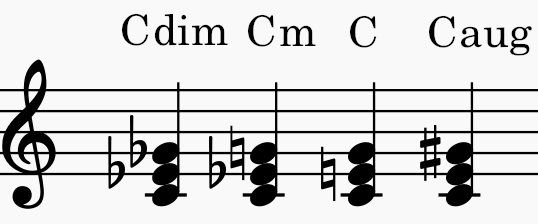
\includegraphics[width=1\linewidth]{resources/triads.png}
        \caption{簡単なコード}
        \label{fig:triads}
    \end{subfigure}
    \begin{subfigure}{0.5\textwidth}
        \centering
        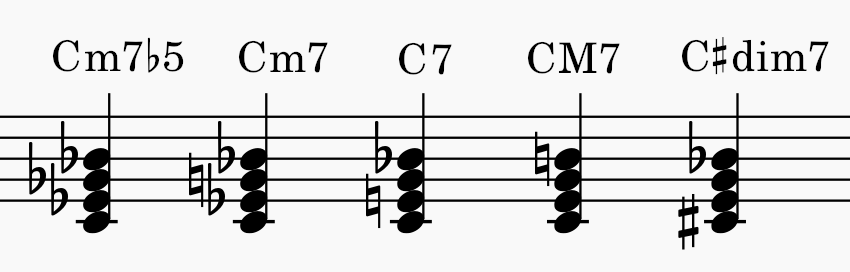
\includegraphics[width=1\linewidth]{resources/seventh chords.png}
        \caption{セブンスコード}
        \label{fig:seventhChords}
    \end{subfigure}
\centering

\end{figure}
\subsubsection{調・キー}
20世紀までの近代西洋音楽では、半音階のすべての音を使わず、同時に使うのは大体そこから七個だけを選んだ部分集合です。この部分集合を調、スケール、音階、あるいはキーと呼びます。簡単に云うと、絵画でいう「パレット」のようなものです。調には一つ基準点として機能する「トニック」が存在し、そこから音程を用いてスケールを定義できます。最も有名なスケールはメジャースケール（長調）で、トニックのM2, M3, P4, P5, M6, M7上の音をチョイスしてパレットが構成されます。ドを基準にしてとっていくと、つまりドレミファソラシ (C, D, E, F, G, A, B)ですね。他にも、東方をやる上では必須な、自然短音階(ナチュラルマイナースケール、natural minor scale)というものもあります。こちらはトニックからM2, m3, P4, P5, m6, m7上の音を選んだものです。Cを基準にして具体的に書いていくと、Cマイナースケール≡C D E\fl , F, G, A\fl , B\fl となります。そして、よくみるものに和声短音階(ハーモニックマイナースケール、harmonic minor scale) というものもあります。こちらはR, M2, m3, P4, P5, m6, M7の構成で、C基準でいくとC D E\fl , F, G, A\fl , B\na です。命名や用途は書き出すと長く語ってしまうので興味のある方は調べてみてください。\par 
キーの中の音を、トニックからの音程をベースに数字を与え、記述することができます。例えば、C majorにおいて、Aは六度目なので\sd{6} と書き表すことができ、C minorで、Fは四度目なので\sd{4}, A\fl は六度目なので\fl \sd{6}と表記することができます（調を明らかにできるように\sd{6}ではなく\sd{b6}と書きました。詳細は付録末にて）。これによって、絶対音感を持たない身分であるせいで、キーが不明であっても、聞こえる音を認識し、記述することができます（例えば、「あ、今\na \sd{7} \sd{2} \sd{1}という旋律が聞こえたな。」と）\par
また、キーという「パレット」に存在しない音を例外的に採用することが存在し、それはよく「臨時記号」と呼ばれます。臨時記号は特異的な雰囲気を纏うことが多く、音楽的な意味が大きく込められていることが多いので、度々分析の対象となります。\par
キーを楽譜上に表すのが「調号」で、これは\trebleclef \bassclef のすぐ右に書かれる\sh や\fl の集まりです。これらは、キーを設定するために選ばれた音の\sh や\fl を因数分解のように「外に括りだして」楽譜を読みやすくするものです。逆に、臨時記号は楽譜途中の\sh や\fl であり、これらは一小節が終わるとリセットされると思って読むと良いでしょう。
\subsubsection{コードの機能}
キーというパレットを定めたうえで、その音を使ってコードというのをつくってみると、例えば、C majorから選んでいくと、C, D, E, F, G, A, Bという音が許されるので、そこから作られるコードは\writechord{C, Dm, Em, F, G, Am, Bdim}となります。逆にC minorから音を選んでつくると、\writechord{Cm, Ddim, Eb, Fm, Gm, Ab, Bb}のコードを作ることができます。こうしてキーの中の音を使って作ったコードをダイアトニックコードと呼びます。ダイアトニックコードは、キーの中ではある特定の雰囲気・役割を持つという基本的な考え方（機能和声という考え方）があり、その理論のもとでは、コードの役割は大きく分けて三つに分類されます：
\begin{itemize}
    \item トニック：安定した響きを持つコードです。イメージでいうと、曲の終わりや、お辞儀の最後です。
    \item ドミナント：不安定な響きを持ち、トニックが次に来ると快楽を覚えさせるコード。ドミナントからトニックコードに向かうことを「解決」と呼びます
    \item サブドミナント（プレドミナント）：トニックに対する解決力は弱いが、ドミナントを持ってくるための下準備・勢い作りを
することができる。癖が強いコードが多い。
\end{itemize}
どのダイアトニックコードがどのような役割を持つのかは付録の最後に説明しています。\par
このコードの役割を理解すると、コード進行は一つの物語を作ることが想像できます。トニックから始まり、サブドミナントで勢いを作り、ドミナントで緊張を作ってトニックに解決するというサイクルは、「起承転結」の音楽版であると云えます。
\subsubsection{ローマ数字表記}
スケールにおける帽子付き数字（スケール度数）と同様に、コードをキーの中での役割によって記述する方法があります。それは、コードのルートのスケール度数を記述することです。これは、コードのキーの中での聞こえ方・役割が、ルートのスケール度数に大方依存するという経験則的大筋から由来します。逆に、同じコードでも、異なる文脈（キー）の中で演奏すれば、その意味や聞こえ方は変わってくるということです。例えば、キーC minorで演奏する\writechord{Gm}はドミナントコードですが、キーD minorで演奏する\writechord{Gm}はサブドミナントであり、全く雰囲気が違います。スケール度数と同様に、ローマ数字を用いることによって、キーを併記しないでコード進行を記述し、記述を一般化することができます。例えば、東方原曲での数多くの曲は「\writechord{bVI bVII i}」（例：キーC minorにおける\writechord{Ab} \wc{Bb} \wc{Cm}, キーD minorにおける \writechord{Bb} \writechord{C Dm}）というコード進行を使っているという事実があります。ローマ数字の振り方は付録の最後にて説明しています。
\subsection{ネオ・リーマン理論について}

\subsection{本稿における表記法と思想}
音楽理論を扱う世のマテリアルでは表記（と流派）が異なることも多いので、本稿で使用する表記とコードの解釈について追記します。特に、東方は短調ベースで書かれることが多く、臨時記号も多用するので、それに適応した表記として、長調としての表記・分析より短調としての表記や分析を行うことが多いと思います。\par
具体的に、コードのルートに対する度数とスケ
ールに対する度数を区別するため、後者をアクセント
付きの数字で表記していきます。（\autoref{fig:scales}）\par
\begin{itemize}
    \item  長音階に関しては \sd{1} \sd{2} \sd{3} \sd{4} \sd{5} \sd{6} \sd{7} と表記
    \item 自然短音階は \sd{1} \sd{2} \fl \sd{3} \sd{4} \sd{5} \fl \sd{6} \fl \sd{7} と表記
    \item その上で、臨時記号をその都度用いる（例: 和声短音階は \sd{1} \sd{2} \fl \sd{3} \sd{4} \sd{5} \fl \sd{6} \na \sd{7} ）
\end{itemize}

\begin{figure}
    \centering
    \begin{subfigure}{0.4\textwidth}
        \centering
        
\includegraphics[width=\linewidth]{resources/major scale.png}
        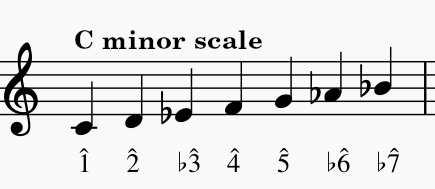
\includegraphics[width=\linewidth]{resources/minor scale.png}
        \caption{長音階、短音階}
        \label{fig:scales}
    \end{subfigure}
    \begin{subfigure}{0.4\textwidth}
        \centering
        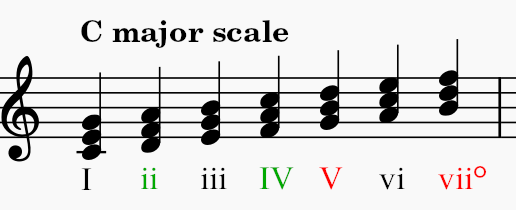
\includegraphics[width=\linewidth]{resources/major scale chords.png}
        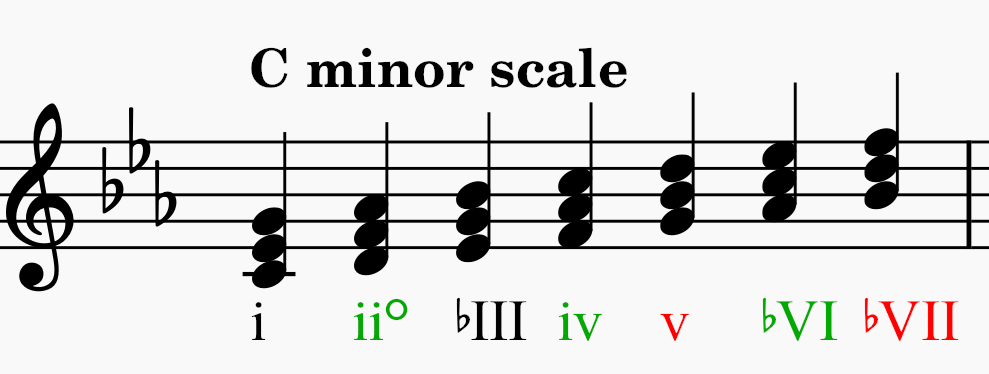
\includegraphics[width=\linewidth]{resources/minor scale chords.png}
        \caption{長音階、短音階のダイアトニックコード}
        \label{fig:diatonicChords}  
    \end{subfigure}
    \caption{本稿での表記}
    \label{fig:notation}
\end{figure}

また、コードのローマ数字表記に関して、メジャーコードとマイナーコードの表記法を区別します。（\autoref{fig:diatonicChords}）
\begin{itemize}
    \item メジャーコードは大文字
    \item マイナーコードは小文字
    \item コードエクステは重要であると判断した場合に表記
\end{itemize}
続いてダイアトニックコードの役割ですが、ダイアトニックコードの役割は教材・ソースによって割れることも多々あるので予めここで本稿においての考えを断っておきます。（\autoref{tab:diatonicFunctions}）
\begin{itemize}
    \item 長調
    \begin{itemize}
        \item \writechord{I}, \writechord{iii}, \writechord{vi}はトニック役  
        \item \writechord{V}, \writechord{viio}はドミナント役
        \item \writechord{ii}, \writechord{IV}はプレドミナント役   
    \end{itemize}
    \item 短調
    \begin{itemize}
        \item \writechord{i}, \writechord{bIII}, \writechord{vi}はトニック役  
        \item \writechord{v}, \writechord{bVII}はドミナント役
        \item \writechord{iio}, \writechord{iv}, \writechord{bVI}はプレドミナント役   
    \end{itemize}
\end{itemize}

\begin{table}
    \centering
    \caption{コードの役割}
    \begin{tabular}{|c|c|c|c|}\hline
        調 & トニック & ドミナント & プレドミナント \\\hline
        長調 & \makecell{\writechord{I} \\ \wc{iii} \\ \wc{vi}} & \makecell{\wc{V} \\ \writechord{viio}} & \makecell{\wc{IV} \\ \wc{ii}} \\
        短調 & \makecell{\writechord{i} \\ \wc{bIII}} & \makecell{\wc{v} \\ \writechord{bVII}} & \makecell{\wc{iv} \\ \writechord{bVI} \\ \wc{iio}} \\ \hline
    \end{tabular}
    \label{tab:diatonicFunctions}
\end{table}

\bibliographystyle{plain}
% \bibliographystyle{aipnum-cp}%
\bibliography{references}

\end{document}
